% Editable three-panel vector schematic. Compile with pdflatex.
\documentclass[tikz,border=3mm]{standalone}
\usepackage[T1]{fontenc}
\usepackage{lmodern}
\usepackage{amsmath,amssymb}
\usetikzlibrary{arrows.meta,calc,positioning}
\begin{document}
\sffamily
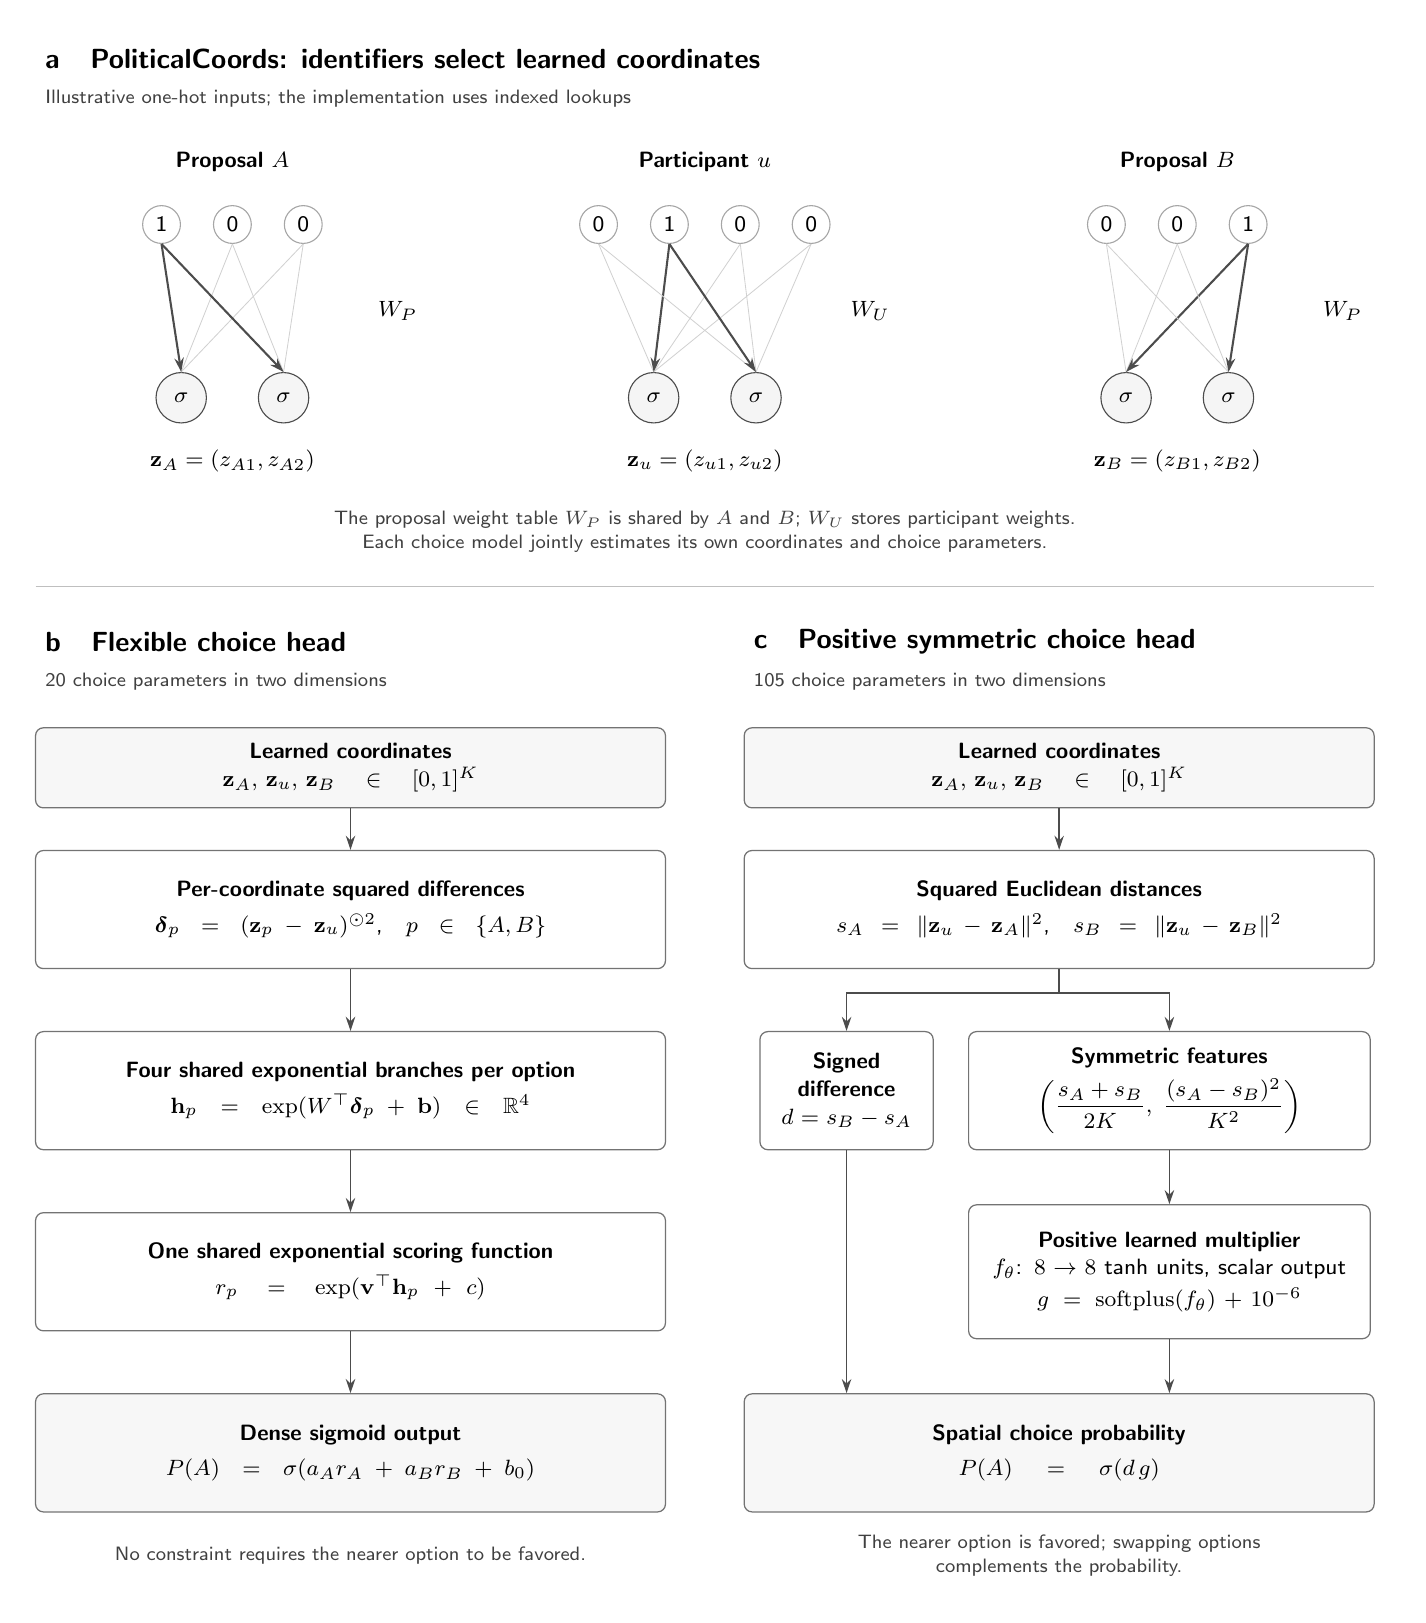
\begin{tikzpicture}[x=1mm,y=1mm,
  font=\sffamily\fontsize{8}{10}\selectfont,
  box/.style={draw=black!55,line width=.45pt,rounded corners=1mm,
              fill=white,align=center,inner sep=2mm},
  common/.style={box,fill=black!3},
  arr/.style={-{Stealth[length=1.8mm,width=1.2mm]},draw=black!70,line width=.55pt},
  hint/.style={font=\sffamily\fontsize{7}{8.7}\selectfont,text=black!75,align=center}]
\useasboundingbox (-1,74) rectangle (173,-125);

% A node view of the common embedding-layer specification. K=2 is illustrative.
\node[anchor=west,font=\sffamily\bfseries\fontsize{10}{12}\selectfont] at (0,70)
  {a\quad PoliticalCoords: identifiers select learned coordinates};
\node[hint,anchor=west] at (0,65)
  {Illustrative one-hot inputs; the implementation uses indexed lookups};
\foreach \xc/\prefix/\who/\wm/\nn/\selected in {
  25/A/Proposal $A$/W_P/3/1,
  85/U/Participant $u$/W_U/4/2,
  145/B/Proposal $B$/W_P/3/3}{
  \node[font=\sffamily\bfseries\fontsize{8}{10}\selectfont] at (\xc,57) {\who};
  \foreach \i in {1,...,\nn}{
    \pgfmathsetmacro{\xx}{\xc+9*(\i-(\nn+1)/2)}
    \node[circle,draw=black!35,fill=white,minimum size=4.8mm,inner sep=0pt]
      (\prefix in\i) at (\xx,49) {\ifnum\i=\selected\relax 1\else 0\fi};
  }
  \foreach \j in {1,2}{
    \pgfmathsetmacro{\xx}{\xc+13*(\j-1.5)}
    \node[circle,draw=black!70,fill=black!4,minimum size=6.4mm,inner sep=0pt]
      (\prefix out\j) at (\xx,27) {$\sigma$};
    \foreach \i in {1,...,\nn}{
      \draw[draw=black!18,line width=.3pt] (\prefix in\i.south) -- (\prefix out\j.north);
    }
    \draw[arr,line width=.75pt] (\prefix in\selected.south) -- (\prefix out\j.north);
  }
  \node[font=\sffamily\fontsize{8}{10}\selectfont,fill=white,inner sep=.5mm]
    at (\xc+21,38) {$\wm$};
}
\node at (25,19) {$\mathbf z_A=(z_{A1},z_{A2})$};
\node at (85,19) {$\mathbf z_u=(z_{u1},z_{u2})$};
\node at (145,19) {$\mathbf z_B=(z_{B1},z_{B2})$};
\node[hint,text width=164mm] at (85,10)
 {The proposal weight table $W_P$ is shared by $A$ and $B$; $W_U$ stores participant weights.\\
  Each choice model jointly estimates its own coordinates and choice parameters.};
\draw[black!25,line width=.35pt] (0,3) -- (170,3);
\node[anchor=west,font=\sffamily\bfseries\fontsize{10}{12}\selectfont] at (0,-4)
 {b\quad Flexible choice head};
\node[anchor=west,font=\sffamily\bfseries\fontsize{10}{12}\selectfont] at (90,-4)
 {c\quad Positive symmetric choice head};
\node[hint,anchor=west] at (0,-9) {20 choice parameters in two dimensions};
\node[hint,anchor=west] at (90,-9) {105 choice parameters in two dimensions};
\foreach \x/\p in {0/a,90/b}{
 \node[common,text width=76mm,minimum height=8mm] (\p embed) at (\x+40,-20)
  {\textbf{Learned coordinates}\\$\mathbf z_A,\,\mathbf z_u,\,\mathbf z_B\in[0,1]^K$};
}
% Flexible head. Squared differences remain coordinate-specific.
\node[box,text width=76mm,minimum height=15mm] (adelta) at (40,-38)
     {\textbf{Per-coordinate squared differences}\\[1mm]
      $\boldsymbol\delta_p=(\mathbf z_p-\mathbf z_u)^{\odot2}$,\quad $p\in\{A,B\}$};
\draw[arr] (aembed.south) -- (adelta.north);
\node[box,text width=76mm,minimum height=15mm] (abranch) at (40,-61)
     {\textbf{Four shared exponential branches per option}\\[1mm]
      $\mathbf h_p=\exp(W^\top\boldsymbol\delta_p+\mathbf b)\in\mathbb R^4$};
\draw[arr] (adelta.south) -- (abranch.north);
\node[box,text width=76mm,minimum height=15mm] (ascore) at (40,-84)
     {\textbf{One shared exponential scoring function}\\[1mm]
      $r_p=\exp(\mathbf v^\top\mathbf h_p+c)$};
\draw[arr] (abranch.south) -- (ascore.north);
\node[common,text width=76mm,minimum height=15mm] (aout) at (40,-107)
     {\textbf{Dense sigmoid output}\\[1mm]
      $P(A)=\sigma(a_A r_A+a_B r_B+b_0)$};
\draw[arr] (ascore.south) -- (aout.north);
% Positive symmetric head. A signed distance difference bypasses the MLP.
\node[box,text width=76mm,minimum height=15mm] (bdist) at (130,-38)
     {\textbf{Squared Euclidean distances}\\[1mm]
      $s_A=\|\mathbf z_u-\mathbf z_A\|^2$,\quad $s_B=\|\mathbf z_u-\mathbf z_B\|^2$};
\draw[arr] (bembed.south) -- (bdist.north);
\node[box,text width=18mm,minimum height=15mm] (bsign) at (103,-61)
     {\textbf{Signed}\\\textbf{difference}\\$d=s_B-s_A$};
\node[box,text width=47mm,minimum height=15mm] (bfeat) at (144,-61)
     {\textbf{Symmetric features}\\[1mm]
      $\displaystyle\left(\frac{s_A+s_B}{2K},\;\frac{(s_A-s_B)^2}{K^2}\right)$};
\draw[arr] (bdist.south) -- ++(0,-3) -| (bsign.north);
\draw[arr] (bdist.south) -- ++(0,-3) -| (bfeat.north);
\node[box,text width=47mm,minimum height=17mm] (bscale) at (144,-84)
     {\textbf{Positive learned multiplier}\\
      $f_\theta$: $8\to8$ tanh units, scalar output\\[.5mm]
      $g=\operatorname{softplus}(f_\theta)+10^{-6}$};
\draw[arr] (bfeat.south) -- (bscale.north);
\node[common,text width=76mm,minimum height=15mm] (bout) at (130,-107)
     {\textbf{Spatial choice probability}\\[1mm]
      $P(A)=\sigma(d\,g)$};
\draw[arr] (bscale.south) -- (bscale.south |- bout.north);
\draw[arr] (bsign.south) -- (bsign.south |- bout.north);
\node[hint,text width=77mm] at (40,-120) {No constraint requires the nearer option to be favored.};
\node[hint,text width=77mm] at (130,-120) {The nearer option is favored; swapping options\\complements the probability.};
\end{tikzpicture}
\end{document}
